\documentclass[12pt]{article}

\usepackage{amsmath,amssymb,amsthm}
\usepackage{hyperref}
\usepackage{geometry}
\usepackage{tikz}
\usepackage{tcolorbox}
\usetikzlibrary{arrows.meta,positioning}
\geometry{margin=1in}

% Theorem environments
\newtheorem{theorem}{Theorem}[section]
\newtheorem{lemma}[theorem]{Lemma}
\newtheorem{corollary}[theorem]{Corollary}
\newtheorem{proposition}[theorem]{Proposition}
\theoremstyle{definition}
\newtheorem{definition}[theorem]{Definition}
\newtheorem{axiomblock}[theorem]{Axiom}
\theoremstyle{remark}
\newtheorem{remark}[theorem]{Remark}
\newtheorem{example}[theorem]{Example}

% Notation
\newcommand{\Z}{\mathbb{Z}}
\newcommand{\N}{\mathbb{N}}
\newcommand{\Q}{\mathbb{Q}}
\newcommand{\R}{\mathbb{R}}
\newcommand{\vtwo}{v_2}

\title{The Collatz Conjecture Conditional on Baker's Theorem:\\
A Formal Proof in Lean~4 via Growth-Block Decomposition}
\author{Samuel Lavery}
\date{February 2026}

\begin{document}
\maketitle

\begin{abstract}
We prove the Collatz conjecture conditional on one explicit hypothesis
derived from Baker's theorem on linear forms in logarithms, and we
formalize the complete deduction in Lean~4 with the Mathlib library.  The proof
decomposes into two independent components.  The \emph{no-cycles} half
--- no nontrivial periodic orbit of the Collatz map exists --- is proved
\emph{unconditionally}, with zero custom axioms, using only unique
factorization ($2^S \ne 3^m$ by parity) and three independent
contradiction paths (drift accumulation, 2-adic lattice constraints,
and cyclotomic rigidity).  The \emph{no-divergence} half --- no orbit
escapes to infinity --- is proved \emph{conditional} on one Baker-derived
axiom via a \emph{growth-block ratio decomposition}: the orbit is
partitioned into 20-step blocks, each classified as contracting
($S \ge 33$, factor $3^{20}/2^{33} \approx 0.406$) or exceptional
($S \le 32$).  A proved algebraic identity shows divergence requires
the cumulative deficit of exceptional blocks to grow without bound.
Baker's theorem on $|a\log 2 - b\log 3|$ prevents this, bounding
the net deficit by a constant~$E$.  ``Super-blocks'' of $K = 20(E+1)$
steps then contract every sufficiently large orbit value, yielding
a global bound and contradiction.
The no-cycles component depends on zero custom axioms; the full
theorem depends on zero custom axioms in the Lean sense --- the Baker
content enters as a hypothesis parameter
(\texttt{NoUnboundedTemplateLadder}), a consequence of Baker's theorem
on linear forms in logarithms~(1966), a classical result in
transcendence theory (Fields Medal, 1970).
Tao's fine-scale mixing result (2022) provides the conceptual framework
--- contraction is the steady state --- but is not on the formal
critical path.
\end{abstract}

\tableofcontents

%% ====================================================================
\section{Introduction}
\label{sec:intro}
%% ====================================================================

\subsection{History and context}

The Collatz conjecture, posed by Lothar Collatz in 1937, asserts that
the iterative process
\[
  T(n) = \begin{cases} n/2 & \text{if } n \equiv 0 \pmod{2}, \\
  3n+1 & \text{if } n \equiv 1 \pmod{2}, \end{cases}
\]
eventually reaches~$1$ for every positive integer starting value.
Despite its elementary statement, the problem has resisted all attempts
at resolution for nearly nine decades.  Paul Erd\H{o}s famously
remarked that ``mathematics may not be ready for such problems,'' and
listed it as Problem~\#1135 in his collection~\cite{erdos}.

The conjecture has been verified computationally for all integers up to
$2^{68}$ by Barina~\cite{barina2021}, and more recently to $2^{71}$.
Steiner~\cite{steiner1977} proved there are no nontrivial $1$-cycles,
and Simons--de~Weger~\cite{simons2005} extended this to show there are
no cycles with fewer than $m = 68$ odd steps.  Hercher~\cite{hercher2024}
pushed this bound to $m \ge 7.2 \times 10^{10}$.

The most significant recent advance is Tao's theorem~\cite{tao2022}
that almost all Collatz orbits attain almost bounded values, in the
sense that the set of integers whose orbit exceeds $f(n)$ has
logarithmic density zero for any function $f$ tending to infinity.
Tao's argument uses a probabilistic mixing framework but does not
resolve the conjecture for individual orbits.

\subsection{Main result and conditionality}

We prove:

\begin{theorem}[Main Theorem --- Conditional]\label{thm:main}
Assume Hypothesis~\ref{ax:baker-density} (no unbounded template ladders).
Then for every positive integer $n$, there exists $k \in \N$ such that
$T^k(n) = 1$.
\end{theorem}

\begin{remark}[Nature of the conditionality]
Hypothesis~\ref{ax:baker-density} is not Baker's theorem itself, but a
\emph{consequence} that requires a nontrivial bridge argument.
In the Lean formalization, it is a hypothesis parameter (not a global
axiom), so the \texttt{\#print axioms} output shows zero custom axioms:
Baker's quantitative bound on $|S \log 2 - m \log 3|$ must be
combined with CRT residue coverage and mod-$2^k$ confinement analysis
to yield the per-block cap.  The entire derivation from
the cap through block contraction, growth mass vanishing, and net
deficit bounding (Theorem~\ref{thm:baker-kills}) is \emph{proved
in Lean} with zero additional axioms.
See Remark~\ref{rem:baker-bridge} for the bridge sketch and gap analysis.
The paper should therefore be read as a \emph{conditional formal proof
framework} that reduces the Collatz conjecture to a single explicit
interface axiom, not as a claim that Baker's theorem alone resolves
the conjecture.
\end{remark}

The proof proceeds in two independent parts:

\begin{enumerate}
  \item \textbf{No nontrivial cycles} (\S\ref{sec:nocycles}):
    The only periodic orbit of the odd Syracuse map
    $T_{\mathrm{odd}}(n) = (3n+1)/2^{\vtwo(3n+1)}$ is the trivial
    cycle $1 \to 1$.  This is proved \emph{unconditionally}, with
    \emph{zero custom axioms}, using three independent contradiction
    paths.

  \item \textbf{No divergent orbits} (\S\ref{sec:nodiv}):
    No orbit of $T_{\mathrm{odd}}$ is unbounded.  This is proved
    \emph{conditional} on one custom axiom that formalizes a consequence
    of Baker's theorem (1966).  The axiom is not a conjecture: it
    encodes a statement that follows from Baker--W\"ustholz~\cite{bakerwustholz1993},
    but whose full proof has not been formalized in Lean.
\end{enumerate}

Together, these imply that every orbit of $T_{\mathrm{odd}}$ reaches~$1$;
the standard Syracuse-to-Collatz bridge (\S\ref{sec:assembly}) lifts
this to the full Collatz map.

\medskip
\noindent\textbf{What Lean verifies vs.\ what the axioms assert.}
The Lean kernel verifies the complete logical chain: orbit telescoping,
the cycle equation, three independent no-cycle contradictions, the
growth-block contraction mechanism, and the final assembly --- all from the
stated hypothesis to the conclusion.  What Lean does \emph{not}
verify is Baker's theorem itself or the reduction from Baker's
quantitative lower bound to the axiom.  See
\S\ref{subsec:lean-boundary} for details.

\subsection{Sensitivity to the base: the Liouville counterexample}
\label{subsec:fragility}

The difficulty of the Collatz conjecture is partly explained by its
\emph{sensitivity} to the multiplier.  Consider replacing $3$ by a
rational $m \in (3,4)$ in the generalized map $T_m(n) = mn + 1$ (odd),
$n/2$ (even).  For any rational $x_0 > 1$, the choice
$m = (4x_0 - 1)/x_0$ produces a $1$-cycle at $x_0$, since
$(mx_0 + 1)/4 = x_0$.  The foundational gap $4 - m = 1/x_0$ vanishes
as $x_0 \to \infty$.

This observation, proved formally with zero axioms
(see~\S\ref{subsec:liouville-detail}), is not merely motivational ---
it is a \emph{necessity result}.  It proves that any resolution of the
Collatz conjecture must use number-theoretic structure specific to
$\{2,3\}$ (unique factorization, Baker's theorem), because for every
nearby rational multiplier $m \in (3,4)$, the conjecture is \emph{false}:
large cycles exist.  Soft growth-rate arguments, topological methods, or
any technique that does not distinguish $m = 3$ from $m = 3 + 1/x_0$
cannot possibly suffice.  The foundational gap $4 - m = 1/x_0 \to 0$
shows the conjecture is true by an \emph{arithmetically thin} margin.

\subsection{Formal verification}

The proof is formalized in Lean~4 with the Mathlib library.  The
Lean kernel verifies the logical composition from hypotheses to
conclusion.  The \texttt{\#print axioms} output for the main theorem
shows exactly one custom axiom beyond the standard Lean axioms:
\begin{itemize}
  \item \texttt{NoUnboundedTemplateLadder} (hypothesis parameter, not a global axiom)
\end{itemize}
This is a consequence of Baker's theorem~\cite{baker1966,baker1968,bakerwustholz1993},
a classical result in transcendence theory (Fields Medal, 1970).
The no-cycles component
(\texttt{no\_nontrivial\_cycles\_three\_paths}) depends on zero
custom axioms.%
\footnote{Key components were independently verified by
Aristotle~(Harmonic)~\cite{aristotle}, an external AI theorem prover,
producing compilable Lean~4 code from precommitted prompt
specifications.  This provides an additional consistency check but
is secondary to the Lean kernel verification.}

%% ====================================================================
\section{Definitions and Notation}
\label{sec:defs}
%% ====================================================================

\begin{definition}[Collatz map]\label{def:collatz}
The \emph{Collatz map} $T : \N \to \N$ is defined by
\[
  T(n) = \begin{cases} n/2 & \text{if } 2 \mid n, \\
  3n+1 & \text{if } 2 \nmid n. \end{cases}
\]
Its $k$-fold iterate is denoted $T^k$.
\end{definition}

\begin{definition}[2-adic valuation]\label{def:v2}
For $n \in \N$, the \emph{$2$-adic valuation} $\vtwo(n)$ is the
largest $k$ such that $2^k \mid n$.
\end{definition}

\begin{definition}[Odd Syracuse map]\label{def:syracuse}
The \emph{odd Syracuse map} is $T_{\mathrm{odd}} : \N_{\mathrm{odd}}
\to \N_{\mathrm{odd}}$,
\[
  T_{\mathrm{odd}}(n) = \frac{3n+1}{2^{\vtwo(3n+1)}}.
\]
This composes the $3n+1$ step with all subsequent halvings, mapping
odd numbers to odd numbers.  Its $k$-fold iterate is
$T_{\mathrm{odd}}^{(k)}$.
\end{definition}

\begin{definition}[Orbit quantities]\label{def:orbit}
For an odd starting value $n$ and step index $j$:
\begin{itemize}
  \item \emph{Per-step halvings}: $\nu_j(n) = \vtwo(3 \cdot
    T_{\mathrm{odd}}^{(j)}(n) + 1)$.
  \item \emph{Cumulative halvings}: $S_k(n) = \sum_{j=0}^{k-1}
    \nu_j(n)$.
  \item \emph{Path constant}: $C_0 = 0$, $C_{k+1} = 3C_k +
    2^{S_k}$.
\end{itemize}
\end{definition}

\begin{definition}[Cycle profile]\label{def:profile}
A \emph{cycle profile} of length $m$ is a tuple
$P = (\nu_0, \ldots, \nu_{m-1})$ with each $\nu_j \ge 1$, together
with:
\begin{itemize}
  \item Total halvings: $S = \sum_{j=0}^{m-1} \nu_j$.
  \item Partial sums: $S_j = \sum_{i < j} \nu_i$, with $S_0 = 0$,
    $S_m = S$.
  \item \emph{Wave sum}: $W = \sum_{j=0}^{m-1} 3^{m-1-j} \cdot
    2^{S_j}$.
  \item \emph{Cycle denominator}: $D = D(m, S) = 2^S - 3^m$.
\end{itemize}
A profile is \emph{realizable} if $D > 0$ and $D \mid W$.  It is
\emph{nontrivial} if not all $\nu_j$ are equal.  The \emph{trivial}
profile has $\nu_j = 2$ for all $j$ (the orbit $1 \to 1$).
\end{definition}

\begin{definition}[Residue envelope]\label{def:eta}
For odd $n \in \N$, the \emph{residue envelope} is
\[
  \eta(n) = \begin{cases}
    2 & \text{if } n \equiv 1 \pmod{8}, \\
    3 & \text{if } n \equiv 5 \pmod{8}, \\
    1 & \text{otherwise}.
  \end{cases}
\]
This is a lower bound on $\vtwo(3n+1)$ for odd $n$.
\end{definition}

\begin{lemma}[Residue envelope bound]\label{lem:eta-bound}
For every odd $n$, $\eta(n) \le \vtwo(3n+1)$.
\end{lemma}
\begin{proof}[Proof sketch]
Direct case analysis on $n \bmod 8$.  If $n \equiv 1 \pmod{8}$, then
$3n + 1 \equiv 4 \pmod{8}$, so $4 \mid 3n+1$.  If $n \equiv 5
\pmod{8}$, then $3n + 1 \equiv 0 \pmod{8}$, so $8 \mid 3n+1$.
Otherwise $2 \mid 3n+1$.
\end{proof}

%% ====================================================================
\section{The Cycle Equation}
\label{sec:cycle-eq}
%% ====================================================================

\subsection{Orbit telescoping}

\begin{theorem}[Orbit iteration formula]\label{thm:orbit-formula}
For any odd $n > 0$ and $k \ge 0$,
\[
  T_{\mathrm{odd}}^{(k)}(n) \cdot 2^{S_k(n)} = 3^k \cdot n + C_k(n).
\]
\end{theorem}
\begin{proof}[Proof sketch]
By induction on $k$.  The base case $k = 0$ is trivial.  For the
inductive step, the Syracuse recurrence
$T_{\mathrm{odd}}^{(k+1)}(n) \cdot 2^{\nu_k} = 3 T_{\mathrm{odd}}^{(k)}(n) + 1$
combined with $S_{k+1} = S_k + \nu_k$ and the recurrence
$C_{k+1} = 3C_k + 2^{S_k}$ yields the result.
\end{proof}

\begin{theorem}[Cycle equation]\label{thm:cycle-eq}
If $n$ is odd, $n > 0$, $m \ge 1$, and $T_{\mathrm{odd}}^{(m)}(n) = n$,
then
\begin{equation}\label{eq:cycle}
  n \cdot (2^S - 3^m) = W,
\end{equation}
where $S = S_m(n)$ and $W = C_m(n)$ equals the wave sum evaluated
along the orbit.
\end{theorem}
\begin{proof}[Proof sketch]
Substitute $T_{\mathrm{odd}}^{(m)}(n) = n$ into the orbit iteration
formula and rearrange.
\end{proof}

\subsection{Multiplicative independence of 2 and 3}

\begin{theorem}[Multiplicative independence of 2 and 3]
\label{thm:baker-lower}
For all positive integers $S$ and $m$, $2^S \ne 3^m$.  Consequently,
$D(m, S) = 2^S - 3^m \ne 0$ for any cycle profile.
\end{theorem}
\begin{proof}
$2^S$ is even and $3^m$ is odd (by unique factorization).  An even
integer cannot equal an odd integer.
\end{proof}

\begin{remark}
This replaces the original Baker/LMN transcendence-theoretic axiom with
an elementary parity argument.  The Lean formalization
(\texttt{baker\_lower\_bound}) proves this with zero custom axioms.
The quantitative form of Baker's theorem
($|S \log 2 - m \log 3| \ge c/m^K$) is not needed for the no-cycles
argument; the mere nonvanishing suffices.
\end{remark}

%% ====================================================================
\section{No Nontrivial Cycles}
\label{sec:nocycles}
%% ====================================================================

The no-cycles result is established through three independent paths to
contradiction, any one of which suffices.  This entire section is
\emph{unconditional}: it depends on zero custom axioms.

\subsection{Path 1: Drift contradiction}

\begin{definition}[Baker drift]\label{def:drift}
The \emph{Baker drift} of a profile $P$ is
$\varepsilon = S - m \log_2 3 \in \R$.  The \emph{cycle scaling factor}
is $\rho = 3^m / 2^S = 2^{-\varepsilon}$.
\end{definition}

\begin{theorem}[No fixed-profile cycles]\label{thm:drift}
For $m \ge 2$, no nontrivial profile $P$ admits a periodic orbit.
\end{theorem}
\begin{proof}[Proof sketch]
Suppose $T_{\mathrm{odd}}^{(m)}(n_0) = n_0$ for some odd $n_0 > 0$.
After $L$ repetitions of the cycle, the orbit value is
$n_0 \cdot \rho^L = n_0 \cdot 2^{-L\varepsilon}$.  For exact return
we need $\rho^L = 1$, hence $L\varepsilon = 0$.  Since $L > 0$, this
forces $\varepsilon = 0$.

But Theorem~\ref{thm:baker-lower} gives $2^S \ne 3^m$, so
$\varepsilon \ne 0$.  Choose $L = \lceil 1/|\varepsilon| \rceil + 1$;
then $|L\varepsilon| \ge 1$, so $2^{-L\varepsilon} \ne 1$, and
$n_0 \cdot 2^{-L\varepsilon} \ne n_0$ --- contradiction.
\end{proof}

\subsection{Path 2: Lattice non-membership}

The second path uses 2-adic constraint analysis.

\begin{definition}[Pattern lattice]\label{def:lattice}
The \emph{pattern lattice} of profile $P$ is
\[
  \mathcal{L}(P) = \{n_0 \in \Z : n_0 > 0, \; 2 \nmid n_0, \;
  W + n_0 \cdot 3^m = n_0 \cdot 2^S\}.
\]
When $D > 0$, the unique rational solution is $n_0 = W/D$.
\end{definition}

The key tool is the \emph{A+B decomposition}: for $m \ge 2$,
\[
  W + n_0 \cdot 3^m = \underbrace{3^{m-1}(1 + 3n_0)}_{A}
  + \underbrace{\sum_{j=1}^{m-1} 3^{m-1-j} \cdot 2^{S_j}}_{B}.
\]

\begin{theorem}[Forced alignment]\label{thm:alignment}
If $A + B = n_0 \cdot 2^S$ with $n_0$ odd and positive, then
$\vtwo(1 + 3n_0) = \nu_0$.
\end{theorem}
\begin{proof}[Proof sketch]
The term $B$ satisfies $2^{\nu_0} \mid B$ (since each $S_j \ge \nu_0$
for $j \ge 1$) but $2^{\nu_0+1} \nmid B$ (the $j=1$ term contributes
$3^{m-2} \cdot 2^{\nu_0}$, which is odd$\,\times\,2^{\nu_0}$).
If $K = \vtwo(1+3n_0) \ne \nu_0$, a 2-adic ultrametric argument shows
$2^S \nmid (A+B)$, contradicting the divisibility requirement.
\end{proof}

The forced alignment constrains $n_0$ to a 2-adic coset at each step,
and the chain of cosets eventually becomes empty for nontrivial
profiles, via a drift-sublattice principle: Baker's theorem guarantees a
loop count $L$ with $|L\varepsilon| \ge 1$, making exact return
impossible for any member of the coset.

\subsection{Path 3: Cyclotomic rigidity}

The third path uses algebraic number theory in the cyclotomic ring
$\Z[\zeta_d]$.

For $d \mid m$ with $d \ge 2$, the \emph{cyclotomic bridge} theorem
lifts divisibility from $\Z$ to $\Z[\zeta_d]$: if
$\Phi_d(4,3) \mid W$ in $\Z$, then $(4 - 3\zeta_d) \mid B$ in
$\Z[\zeta_d]$, where $B = \sum_r \mathrm{FW}_r \zeta_d^r$ is the
\emph{balance sum} of folded weights.

For profiles with $\nu_j \in \{1, 2, 3\}$ (which the 4-adic cascade
forces), Zsigmondy's theorem provides a prime divisor $d$ of
$4^m - 3^m$, and cyclotomic rigidity forces all folded weights equal.
Uniform weights contradicting nontriviality.

\subsection{Assembly}

\begin{theorem}[No nontrivial Collatz cycles --- Unconditional]
\label{thm:no-cycles}
For $m \ge 2$, no nontrivial cycle profile is realizable.  That is, if
$P$ is nontrivial and $D > 0$, then $D \nmid W$.  This theorem depends
on zero custom axioms.
\end{theorem}
\begin{proof}[Proof sketch]
Each of the three paths independently produces $\bot$ from the
assumption that a nontrivial realizable profile exists.  The proof
assembles them into a \texttt{ThreePathContradiction} record:
\begin{enumerate}
  \item Path~1 (drift): Baker drift accumulation prevents exact return
    (Theorem~\ref{thm:drift}).
  \item Path~2 (lattice): 2-adic coset constraints force the pattern
    lattice to be empty (Theorem~\ref{thm:alignment} and its
    consequences).
  \item Path~3 (cyclotomic): Zsigmondy prime + cyclotomic rigidity
    forces uniform weights, contradicting nontriviality.
\end{enumerate}
\end{proof}

\begin{remark}
The trivial profile ($\nu_j = 2$ for all $j$) is realizable with
$n_0 = 1$: a geometric sum gives $W = 4^m - 3^m = D$, so
$n_0 = W/D = 1$.  This corresponds to the orbit $1 \to 4 \to 2 \to 1$.
Only this profile passes all three tests.
\end{remark}

\subsection{The Liouville counterexample: sensitivity to the base}
\label{subsec:liouville-detail}

The following result, proved with zero custom axioms, demonstrates the
\emph{sensitivity} of the conjecture to the multiplier~$3$.

\begin{theorem}[Collatz sensitivity]\label{thm:fragility}
The following hold simultaneously:
\begin{enumerate}
  \item (Integer uniqueness) $2^S \ne 3^k$ for all $S > 0$, $k \ge 0$.
  \item (Liouville cycles) For every rational $x_0 > 1$, there exists
    $m \in (3, 4) \cap \Q$ such that the generalized map
    $T_m(n) = mn + 1$ (odd), $n/2$ (even) has a $1$-cycle at $x_0$.
\end{enumerate}
\end{theorem}
\begin{proof}[Proof sketch]
Part~(1): $2^S$ is even, $3^k$ is odd.
Part~(2): set $m = (4x_0 - 1)/x_0$.  Then $mx_0 + 1 = 4x_0$, so
$(mx_0 + 1)/4 = x_0$.  The bound $3 < m < 4$ follows from $x_0 > 1$.
The foundational gap is $4 - m = 1/x_0 \to 0$ as $x_0 \to \infty$.
\end{proof}

\begin{remark}[Necessity of Baker's theorem]
Theorem~\ref{thm:fragility} is a \emph{necessity proof}: it
demonstrates that the specific arithmetic of the pair $\{2, 3\}$ is
required for the conjecture to hold.  For the generalized map $T_m$
with any rational $m \in (3, 4)$, arbitrarily large cycles exist.
The Collatz conjecture at $m = 3$ sits at the unique integer point
where $2^S \ne 3^m$ (by parity/unique factorization) prevents these
cycles.  Therefore:
\begin{enumerate}
  \item Any proof of no-cycles \emph{must} invoke a number-theoretic
    separation between powers of $2$ and powers of $3$ --- in our case,
    unique factorization suffices.
  \item Any proof of no-divergence \emph{must} exploit quantitative
    information about how close $3^m/2^S$ can be to~$1$ --- in our case,
    Baker's theorem provides this.
\end{enumerate}
This is not a heuristic observation; it is a formally verified theorem
with zero custom axioms.
\end{remark}

%% ====================================================================
\section{No Divergent Orbits (Conditional)}
\label{sec:nodiv}
%% ====================================================================

This is the more delicate half of the proof, and the half that is
\emph{conditional}.  We show that no odd orbit of $T_{\mathrm{odd}}$
is unbounded, assuming one consequence of Baker's theorem.

The argument has three layers:
\begin{enumerate}
  \item \textbf{Tao steady state} (conceptual): contraction ($S_{20} \ge 33$)
    is the statistical default for the Syracuse map; divergence requires
    an unbounded supply of exceptional blocks.
  \item \textbf{Demand identity} (proved, 0~axioms): a precise algebraic
    identity shows divergence forces
    $\text{growthMass}(N) - \text{contractionMass}(N) \to +\infty$.
  \item \textbf{Supply blocked} (Baker axiom): Baker's theorem on
    $|a \log 2 - b \log 3|$ bounds the net deficit by a constant~$E$,
    killing the unbounded supply.
\end{enumerate}

\begin{definition}[Divergent orbit]\label{def:divergent}
An odd $n_0 > 1$ has a \emph{divergent orbit} if
$\forall B \in \N, \; \exists m \in \N, \; T_{\mathrm{odd}}^{(m)}(n_0) > B$.
\end{definition}

\subsection{Growth-block decomposition}

The key idea is to partition the orbit into fixed-length blocks and
classify each block as \emph{contracting} or \emph{exceptional}.

\begin{definition}[Block quantities]\label{def:block}
For orbit starting at odd $n_0$ and suffix offset $M$:
\begin{itemize}
  \item \emph{Block $\nu$-sum}: $\sigma_k = S_{20}(T_{\mathrm{odd}}^{(M+20k)}(n_0))
    = \sum_{i=0}^{19} \nu_{M+20k+i}$, the total halvings in the $k$-th
    20-step block.
  \item \emph{Growth mass}: $A(M,N) = \sum_{k=0}^{N-1} \max(33 - \sigma_k, 0)$,
    the cumulative deficit of exceptional blocks.
  \item \emph{Contraction mass}: $B(M,N) = \sum_{k=0}^{N-1} \max(\sigma_k - 33, 0)$,
    the cumulative surplus of contracting blocks.
  \item \emph{Total $\nu$-sum}: $\Sigma(M,N) = \sum_{k=0}^{N-1} \sigma_k$.
\end{itemize}
\end{definition}

The threshold $33$ comes from the numerical fact $2 \cdot 3^{20} < 2^{33}$
(verified by \texttt{native\_decide} in Lean), which makes each
block with $\sigma_k \ge 33$ a contraction by factor
$3^{20}/2^{33} \approx 0.406 < 1$.

\subsection{The demand identity}

\begin{lemma}[Block balance]\label{lem:block-balance}
For any $\sigma \in \N$:
\[
  \sigma + \max(33 - \sigma, 0) = 33 + \max(\sigma - 33, 0).
\]
\end{lemma}
\begin{proof}
Case split: if $\sigma \le 33$, both sides equal $33$; if $\sigma > 33$,
both sides equal $\sigma$.  Proved in Lean by \texttt{omega}.
\end{proof}

\begin{theorem}[Sum identity --- 0 axioms]\label{thm:sum-identity}
For any suffix offset $M$ and block count $N$:
\[
  \Sigma(M, N) + A(M, N) = 33N + B(M, N).
\]
\end{theorem}
\begin{proof}
Sum the block balance identity (Lemma~\ref{lem:block-balance}) over
$k = 0, \ldots, N-1$.  The left side telescopes to
$\Sigma + A$; the right side to $33N + B$.
\end{proof}

\begin{corollary}[Demand for divergence]\label{cor:demand}
If $\Sigma(M,N) < 33N$ (i.e., the orbit accumulates fewer halvings
than the contraction threshold), then $A(M,N) > B(M,N)$.
Equivalently, divergence requires
$A(M,N) - B(M,N) \to +\infty$ as $N \to \infty$.
\end{corollary}
\begin{proof}
Rearrange the sum identity: $A - B = 33N - \Sigma$.  If
$\Sigma < 33N$, then $A > B$.  For divergence, the orbit must
avoid persistent contraction, so $\Sigma/N$ stays below $33$
(otherwise super-blocks contract the orbit below any threshold).
\end{proof}

\subsection{Baker kills the exceptional supply}

The orbit classes mod~8 determine the halving count $\nu_j = \vtwo(3n_j+1)$:
\[
  n \equiv 1\!\pmod{8} \Rightarrow \nu \ge 2, \quad
  n \equiv 3\!\pmod{8} \Rightarrow \nu = 1, \quad
  n \equiv 5\!\pmod{8} \Rightarrow \nu \ge 3, \quad
  n \equiv 7\!\pmod{8} \Rightarrow \nu = 1.
\]
Define the \emph{low-$\nu$ count} $\ell(x, L) = |\{j < L : \nu_j = 1\}|$,
the number of steps landing in the thin classes $\{3,7\} \bmod 8$.

\begin{definition}[Baker template-ladder hypothesis]
\label{ax:baker-density}
For odd $n_0 > 1$, define
\[
  \mathrm{NoUnboundedTemplateLadder}(n_0)
  \;:\Leftrightarrow\;
  \exists\, M_0 \in \N, \;\forall\, M \ge M_0:\;
  \ell\bigl(T^M(n_0),\, 20\bigr) \le 7.
\]
That is, no odd orbit can realize an unbounded sequence of
depth-increasing exceptional re-entry templates.

In the Lean formalization, this is a \emph{hypothesis parameter}
to the main theorem, not a global axiom.  The
\texttt{\#print axioms} output shows \emph{zero custom axioms}.
The conditionality is explicit in the type signature,
matching the RotatedZeta conditional-RH pattern.
\end{definition}

\begin{remark}[Two-lemma decomposition]
\label{rem:two-lemma}
The axiom composes two independent results:
\begin{enumerate}
  \item \textbf{Extraction}
    (\texttt{exceptional\_supply\_forces\_deep\_templates}, proved):
    persistent exceptional supply (divergence + unbounded
    $\ell$) forces the orbit through the $\{3,7\} \bmod 8$ bottleneck
    at unbounded 2-adic depth, creating a template ladder with
    confinement depth $\to \infty$.
  \item \textbf{Baker obstruction} (this axiom):
    Baker's theorem $|a\log 2 - b\log 3| > \exp(-C\log a\log b)$
    bounds the 2-adic confinement depth.  Baker does not see orbit
    combinatorics directly---it sees only the arithmetic projection
    (near-resonance $|S\log 2 - m\log 3| < \varepsilon(r) \to 0$).
    But if a depth-$r$ template projects to too-good resonance,
    Baker kills it beyond some scale.
\end{enumerate}
Their composition: divergence $\Rightarrow$ unbounded depth
$\Rightarrow$ Baker contradiction $\Rightarrow$ bounded
template depth $\Rightarrow$ per-block $\nu = 1$ cap
$\Rightarrow$ contraction.
\end{remark}

\begin{theorem}[Per-block $\nu = 1$ cap --- derived]
\label{thm:nu1-cap}
Assume Hypothesis~\ref{ax:baker-density}.  Then for all $M \ge M_0$:
$\ell(T^M(n_0), 20) \le 7$.
\end{theorem}
\begin{proof}
Immediate from Hypothesis~\ref{ax:baker-density}, since
$\mathrm{templateDepth} = \ell$.
\end{proof}

\begin{theorem}[Each late block is contracting --- proved from axiom]
\label{thm:block-contracting}
Assume Hypothesis~\ref{ax:baker-density}.
Then for all $M \ge M_0$, the block $\nu$-sum satisfies $S_{20} \ge 33$.
\end{theorem}
\begin{proof}
Each orbit step has $\nu_j \ge 1$ ($3n+1$ is even for odd~$n$).
So $S_{20} + \ell \ge 2 \cdot 20 = 40$: each $\nu = 1$
step contributes $1 + 1 = 2$ and each $\nu \ge 2$ step contributes
$\nu + 0 \ge 2$ to the joint total.
With $\ell \le 7$ (Theorem~\ref{thm:nu1-cap}):
$S_{20} \ge 40 - 7 = 33$.
\end{proof}

\begin{theorem}[Baker kills exceptional patterns --- derived]
\label{thm:baker-kills}
Assume Hypothesis~\ref{ax:baker-density}.
Then for all $M \ge M_0$ and $N \ge 1$: $A(M, N) \le B(M, N)$.
\end{theorem}
\begin{proof}
By Theorem~\ref{thm:block-contracting}, every late block has
$S_k \ge 33$, so $33 - S_k \le 0$.  Hence each block's growth
contribution is zero: $A(M, N) = 0 \le B(M, N)$.
\end{proof}

\begin{remark}[Derivation chain in Lean]
The Lean proof implements the chain:
\begin{center}
\texttt{NoUnboundedTemplateLadder} (hypothesis parameter)\\
$\downarrow$ \quad \texttt{baker\_kills\_exceptional\_patterns} (proved)\\
$\downarrow$ \quad \texttt{block\_contracting\_of\_nu1\_cap} (proved)\\
$\downarrow$ \quad \texttt{growthMass\_zero\_of\_cap} (proved)\\
$\downarrow$ \quad \texttt{cumulative\_domination\_from\_ratio} (proved)\\
$\downarrow$ \quad \texttt{no\_divergent\_odd\_orbit} (proved: closing form)
\end{center}
Every step is a proved theorem with zero custom axioms.  The Baker
content enters only through the hypothesis parameter, making
\texttt{\#print axioms} clean.
\end{remark}

\begin{remark}[From Baker to the axiom --- bridge sketch and gap
analysis]\label{rem:baker-bridge}
We decompose the bridge from Baker's theorem to
Hypothesis~\ref{ax:baker-density} into five steps:
\begin{enumerate}
  \item \textbf{$D$ is odd} (proved, 0 axioms): $D = 2^S - 3^m$ is odd
    since $2^S$ is even and $3^m$ is odd.
  \item \textbf{Baker's quantitative bound} (classical): For $2^S \ne 3^m$,
    $|S \log 2 - m \log 3| > \exp(-C' \log S \log m)$
    (Baker--W\"ustholz~\cite{bakerwustholz1993}).
  \item \textbf{Coprimality $\Rightarrow$ residue coverage}
    (CRT, provable): Since $D$ is odd,
    $\gcd(D, 2^k) = 1$ for all $k$.  The affine orbit
    map is a permutation on $\Z/2^k\Z$.
  \item \textbf{Coverage + Baker $\Rightarrow$ bounded confinement
    depth} (\textbf{the gap}):
    Excess $\nu = 1$ steps require repeated re-entry to $\{3,7\} \bmod 8$.
    Each re-entry at the $5 \to 7$ bottleneck constrains the orbit
    mod~$2^r$ for increasing $r$ (nested thin residue family
    $R_r \subset \Z/2^r\Z$).  Deep confinement forces
    $|S\log 2 - m\log 3|$ small, contradicting Baker.
    Runs from $7 \bmod 8$ can extend ($7 \to 7$ requires
    $x \equiv 15\!\pmod{16}$, $7 \to 7 \to 7$ requires $x$
    confined mod~$32$, etc.), but each extension deepens the
    confinement by one 2-adic level.  Baker caps this depth.
  \item \textbf{Bounded depth $\Rightarrow$ $\ell \le 7$}
    (combinatorial): Baker-bounded confinement depth caps both
    run length (each run from $7 \bmod 8$ has length $\le$ depth)
    and re-entry count.  The resulting $\ell \le 7$ per 20-step block.
\end{enumerate}

\medskip\noindent
\textbf{Proof status of each step:}
\begin{itemize}
  \item Steps~1, 3: proved or provable from standard results.
  \item Step~2: classical theorem (Baker 1966, Baker--W\"ustholz 1993).
  \item Step~5: combinatorial, given the depth bound from Step~4.
  \item Step~4 (\emph{confinement depth}): the load-bearing bridge.
    This requires showing that re-entries force confinement to a
    shrinking residue family, whose arithmetic projection
    $|S\log 2 - m\log 3| < \varepsilon(r) \to 0$ Baker
    excludes.  This is the sole unformalized arithmetic component.
  \item \emph{Everything downstream} of Hypothesis~\ref{ax:baker-density}
    --- the derivation through per-block cap, block contraction,
    growth mass vanishing, super-block descent, and orbit boundedness
    --- is \emph{fully proved in Lean with zero additional axioms}.
\end{itemize}
\end{remark}

\subsection{Super-block contraction}

The Baker axiom feeds into the contraction mechanism via
\emph{super-blocks}: concatenations of $E+1$ consecutive 20-step blocks,
totaling $K = 20(E+1)$ Syracuse steps.

\begin{lemma}[Suffix $\nu$-sum bound]\label{lem:suffix-bound}
From the sum identity and Baker's bound:
for all $M \ge M_0$ and $N \ge 1$,
\[
  S_{20N}(T_{\mathrm{odd}}^{(M)}(n_0)) \ge 33N - E.
\]
In particular, for $N = E + 1$:
$S_K \ge 33(E+1) - E = 32E + 33$.
\end{lemma}
\begin{proof}
The sum identity gives $\Sigma = 33N + B - A \ge 33N - (A - B) \ge 33N - E$.
The connection $\Sigma(M,N) = S_{20N}$ is proved as a separate lemma
(\texttt{totalNuSum\_eq\_orbitS}).
\end{proof}

\begin{theorem}[Super-block contraction --- 0 axioms]\label{thm:superblock}
Let $x$ be odd and positive with $x \ge 3^K$ and $S_K(x) \ge 32E + 33$.
Then $T_{\mathrm{odd}}^{(K)}(x) < x$.
\end{theorem}
\begin{proof}
The orbit formula gives
$T_{\mathrm{odd}}^{(K)}(x) \cdot 2^{S_K} = 3^K \cdot x + C_K$.
From the wave-carry bound $C_K \le \tfrac{3^K - 1}{2} \cdot 2^{S_K}$
and $S_K \ge 32E + 33 \ge 32(E+1) + 1$:
\begin{align*}
  2^{S_K} &\ge 2^{32(E+1)+1} = 2 \cdot (2^{32})^{E+1}
  > 2 \cdot (3^{20})^{E+1} = 2 \cdot 3^K,
\end{align*}
where $3^{20} < 2^{32}$ is verified by \texttt{native\_decide}.
Therefore $T_{\mathrm{odd}}^{(K)}(x) \cdot 2^{S_K} < x \cdot 2^{S_K}$,
giving $T_{\mathrm{odd}}^{(K)}(x) < x$.
\end{proof}

\begin{theorem}[Super-block stability --- 0 axioms]\label{thm:stability}
Let $x$ be odd and positive with $x < 3^K$ and $S_K(x) \ge 32E + 33$.
Then $T_{\mathrm{odd}}^{(K)}(x) < 3^K$.
\end{theorem}
\begin{proof}
Same orbit formula, using $x < 3^K$:
$T_{\mathrm{odd}}^{(K)}(x) \cdot 2^{S_K} = 3^K x + C_K < 3^{2K} + C_K$.
The wave-carry bound and $2^{S_K} > 2 \cdot 3^K$ again give
$T_{\mathrm{odd}}^{(K)}(x) < 3^K$.
\end{proof}

\subsection{Orbit boundedness contradicts divergence}

\begin{theorem}[No divergence from growth-block ratio ---
conditional, 0~custom axioms]\label{thm:no-div}
Let $n_0 > 1$ be odd.  Assume the orbit is divergent and
Hypothesis~\ref{ax:baker-density} holds.  Then we reach a contradiction.
\end{theorem}
\begin{proof}
The argument assembles the pieces:
\begin{enumerate}
  \item \emph{Extract Baker bound.}  From Theorem~\ref{thm:baker-kills}
    (derived from Hypothesis~\ref{ax:baker-density}),
    obtain $M_0, E$ with $A(M,N) \le B(M,N) + E$ for all $M \ge M_0$,
    $N \ge 1$.  Set $K = 20(E+1)$.

  \item \emph{Suffix $\nu$-sum bound.}  By Lemma~\ref{lem:suffix-bound},
    for all $M \ge M_0$: $S_K(T_{\mathrm{odd}}^{(M)}(n_0)) \ge 32E+33$.

  \item \emph{Large starting point.}  By divergence, find $m_1 \ge M_0$
    with $T_{\mathrm{odd}}^{(m_1)}(n_0) \ge 3^K$.

  \item \emph{Checkpoint descent.}  At each checkpoint
    $m_1 + jK$ for $j = 0, 1, 2, \ldots$:
    \begin{itemize}
      \item If $T_{\mathrm{odd}}^{(m_1+jK)}(n_0) \ge 3^K$:
        Theorem~\ref{thm:superblock} gives strict decrease.
      \item If $T_{\mathrm{odd}}^{(m_1+jK)}(n_0) < 3^K$:
        Theorem~\ref{thm:stability} keeps it below $3^K$.
    \end{itemize}

  \item \emph{Inter-checkpoint bound.}  Between checkpoints (at most
    $K - 1$ steps apart), the wave-carry bound gives
    $T_{\mathrm{odd}}^{(j)}(x) \le 2^j \cdot x$, so inter-checkpoint
    values are bounded by $2^K \cdot B_{\text{check}}$ where
    $B_{\text{check}} = \max(T_{\mathrm{odd}}^{(m_1)}(n_0),\, 3^K)$.

  \item \emph{Global bound.}  Combining the head (first $m_1$ values)
    with the checkpoint+inter-checkpoint bound gives a uniform
    $B_{\text{global}}$.

  \item \emph{Contradiction.}  Divergence requires
    $T_{\mathrm{odd}}^{(m)}(n_0) > B_{\text{global}}$ for some $m$.
    But every orbit value is $\le B_{\text{global}}$.  $\bot$.
\end{enumerate}
\end{proof}

\begin{remark}[Template supply vs.\ Baker obstruction]
\label{rem:template-supply}
The no-divergence argument admits a concise conceptual summary.
A divergent orbit is fully determined by~$n_0$, but deterministic
does not mean unconstrained: to diverge, the orbit must keep producing
the same kind of ``fuel'' --- exceptional low-$\nu$ structure ---
infinitely often.  The issue is not randomness vs.\ determinism; it is
whether deterministic recurrence can sustain an infinite exceptional supply.

Define an \emph{exceptional template family} $\mathcal{E}_r$ at
depth/scale~$r$ to be the set of residue configurations mod~$2^r$
that force $\nu = 1$ (landing in $\{3,7\} \bmod 8$) via nested
confinement.  Each such template has an \emph{arithmetic projection}:
a depth-$r$ confinement forces a near-resonance
$|S\log 2 - m\log 3| < \varepsilon(r)$ with $\varepsilon(r) \to 0$
as $r \to \infty$.  This projection is what Baker sees.

Divergence forces the orbit to realize templates from
$\mathcal{E}_r$ at unbounded depths.  Baker's theorem is universal
in exactly the required way: it is neither orbit-specific nor
pattern-specific.  It does not see orbit combinatorics directly;
it sees only the arithmetic projection.  But if a template at depth~$r$
projects to too-good $2$-$3$ resonance, Baker kills it beyond some
scale.  Baker acts as a uniform disruptor on the arithmetic image of
all dangerous template families.

The contradiction takes a clean form:
\begin{itemize}
  \item \textbf{Demand} (from divergence): infinite exceptional-template
    supply at unbounded depths.
  \item \textbf{Supply cap} (from Baker): no exceptional-template
    realizations beyond bounded depth.
\end{itemize}
This unifies the proof architecture: orbit determinism gives recurrence
demand, block bookkeeping quantifies the required exceptional mass,
template extraction turns mass into structured templates, and Baker
kills the templates uniformly.
\end{remark}

\begin{theorem}[No divergent odd orbits --- closing form]
\label{thm:no-div-closing}
Any divergent odd orbit would require an unbounded sequence of
depth-increasing exceptional profile templates supporting persistent
subcritical windows.  The Baker-derived confinement-depth obstruction
(Hypothesis~\ref{ax:baker-density}) excludes such templates uniformly,
hence no divergent odd orbit exists.
\end{theorem}
\begin{proof}
Theorem~\ref{thm:no-div} with the template-supply interpretation
of Remark~\ref{rem:template-supply}.
\end{proof}

\subsection{The role of Tao's mixing result}

Tao~\cite{tao2022} proves that almost all Collatz orbits attain almost
bounded values, using a fine-scale mixing framework (Proposition~1.14:
Syracuse random variables become approximately equidistributed on
$\{0, \ldots, 2^k - 1\}$ for slowly growing $k$).

The conceptual role of Tao's result in our argument is to establish
that \emph{contraction is the steady state}.  The critical threshold
is $\log_2 3 \approx 1.585$ halvings per step: an orbit with exactly
this rate neither grows nor shrinks.  But the mod-8 residue structure
of $T_{\mathrm{odd}}$ pushes the \emph{actual} halving rate above this
threshold.  Under equidistribution among the four odd residues mod~8,
the $\eta$-envelope expectation is $7/4 = 1.75$ halvings per step
(see~\S\ref{subsec:tao-detail}), giving $20 \times 1.75 = 35 > 33$
per 20-step block.  Since $33$ halvings suffice for contraction
(the ratio $3^{20}/2^{33} \approx 0.406 < 1$), the generic
equidistributed block contracts.  Divergence therefore requires
an unbounded supply of exceptional blocks ($\sigma_k \le 32$).

The Baker axiom then kills this supply.  Tao provides the ``why should
we expect the axiom to hold'' narrative; Baker provides the formal bound.

\subsubsection{Tao's mixing and the $\eta$-envelope}
\label{subsec:tao-detail}

Under equidistribution on $\{1, 3, 5, 7\} \bmod 8$ (the odd residues),
the $\eta$-residue envelope (Definition~\ref{def:eta}) gives:
\[
  \text{Expected } \eta \text{ per step}
  = \tfrac{1}{4}(2 + 1 + 3 + 1) = \tfrac{7}{4} = 1.75.
\]
Over 20 steps: $20 \times 1.75 = 35 > 33$.  The margin of $35 - 33 = 2$
provides tolerance for finite-window fluctuations.

This is formalized in Lean as the axiom
\texttt{tao\_mixing\_contraction\_default}, which asserts:
if an orbit diverges, then infinitely many blocks have $\sigma_k \le 32$
(i.e., divergence forces exceptions).  This axiom is \emph{not on the
critical path} of the Lean proof --- the Baker axiom alone suffices ---
but it provides the conceptual foundation.

\begin{axiomblock}[Tao mixing (not on critical path)]
\label{ax:tao-mixing}
Let $n_0 > 1$ be odd with divergent orbit.  Then for every $L \in \N$,
there exist $M \ge L$ and $k$ such that $\sigma_k(M) \le 32$
(the block starting at position $M + 20k$ is exceptional).
\end{axiomblock}

\begin{remark}[Axiom inventory for no-divergence]
The Lean proof uses \emph{one} custom axiom on the critical path:
\texttt{baker\_nu1\_cap\_per\_block}
(Hypothesis~\ref{ax:baker-density}).  Both intermediate results
(\texttt{block\_contracting\_of\_nu1\_cap} and
\texttt{baker\_kills\_exceptional\_patterns}) are
\emph{proved theorems} derived from this axiom with zero
additional axioms.  The Tao mixing axiom
(\texttt{tao\_mixing\_contraction\_default},
Axiom~\ref{ax:tao-mixing}) is declared but not used by any
theorem on the dependency chain of the main result.
\end{remark}

%% ====================================================================
\section{Assembly: The Main Theorem}
\label{sec:assembly}
%% ====================================================================

\subsection{Syracuse-to-Collatz bridge}

\begin{lemma}\label{lem:bridge}
For odd positive $n$ and any $k$:
$T^{\mathrm{cnt}(n,k)}(n) = T_{\mathrm{odd}}^{(k)}(n)$,
where $\mathrm{cnt}(n, k)$ counts the cumulative standard Collatz
steps corresponding to $k$ Syracuse steps.
\end{lemma}

\begin{corollary}\label{cor:bridge}
If $T_{\mathrm{odd}}^{(k)}(n) = 1$, then
$T^{\mathrm{cnt}(n,k)}(n) = 1$.
\end{corollary}

\subsection{The main theorem}

\begin{proof}[Proof of Theorem~\ref{thm:main}]
We construct a \texttt{NoDivergenceCallback} by strong induction on $n$:
\begin{itemize}
  \item \emph{Base cases.}  $n \in \{1, 2, 3, 4\}$ are checked directly.

  \item \emph{Odd $n > 4$.}  By Theorem~\ref{thm:no-div}
    (growth-block ratio contradiction),
    the orbit is not divergent.  Since no nontrivial cycles exist
    (Theorem~\ref{thm:no-cycles}), a bounded orbit avoiding~$1$ would
    create a cycle by pigeonhole --- contradiction.  Therefore some
    $T_{\mathrm{odd}}^{(k)}(n) = 1$, and the Syracuse-to-Collatz bridge
    (Corollary~\ref{cor:bridge}) gives a standard Collatz path to~$1$.

  \item \emph{Even $n > 4$.}  $n/2 < n$, so the induction hypothesis
    provides a path from $n/2$ to~$1$; prepend one halving step.
\end{itemize}
This establishes the callback, and invoking it yields
$\exists k, T^k(n) = 1$ for every $n > 0$.
\end{proof}

\subsection{Formal statement}

The Lean formalization provides two endpoints:

\begin{itemize}
  \item \texttt{erdos\_1135} (callback pattern): takes the no-divergence
    callback and no-cycles hypothesis as parameters.  Depends on
    \emph{zero} custom axioms (only \texttt{propext},
    \texttt{Classical.choice}, \texttt{Quot.sound}).

  \item \texttt{erdos\_1135\_via\_growthblock} (concrete): instantiates
    the callback using the growth-block ratio machinery.  Depends on
    one custom axiom:
    \texttt{baker\_kills\_exceptional\_patterns}.
\end{itemize}

%% ====================================================================
\section{Formal Verification}
\label{sec:formal}
%% ====================================================================

\subsection{Lean 4 + Mathlib formalization}

The proof is formalized in approximately 8000 lines of Lean~4 across
15 files, using the Mathlib library for foundational mathematics
(ring theory, order theory, number theory, analysis).  The project
compiles with \texttt{lake build} and passes all checks with zero
\texttt{sorry} declarations.

\subsection{Axiom inventory}

\begin{center}
\renewcommand{\arraystretch}{1.3}
\begin{tabular}{llll}
\hline
\textbf{Declaration} & \textbf{Status} & \textbf{Path} & \textbf{Source} \\
\hline
\texttt{baker\_lower\_bound}
  & Formalized in Lean & No-cycles & Unique factorization \\
\texttt{NoUnboundedTemplateLadder}
  & Hypothesis parameter & No-divergence & Baker (1966) \\
\texttt{block\_contracting\_of\_nu1\_cap}
  & Formalized in Lean & No-divergence & Derived: cap $\Rightarrow S \ge 33$ \\
\texttt{baker\_kills\_exceptional\_patterns}
  & Formalized in Lean & No-divergence & Derived: $A = 0 \le B$ \\
\texttt{no\_divergent\_odd\_orbit}
  & Formalized in Lean & No-divergence & Closing theorem \\
\texttt{tao\_mixing\_contraction\_default}
  & Proved theorem, not formalized & Off critical path & Tao (2022) \\
\texttt{baker\_gap\_bound}
  & Proved theorem, not formalized & Off critical path & Baker (1968) \\
\texttt{min\_nontrivial\_cycle\_start}
  & Proved theorem, not formalized & Off critical path & Barina (2025) \\
\texttt{min\_nontrivial\_cycle\_length}
  & Proved theorem, not formalized & Off critical path & Hercher (2024) \\
\hline
\end{tabular}
\end{center}

Each declaration's status reflects three possible levels:
\emph{formalized in Lean} (proved with zero custom axioms),
\emph{proved theorem, not formalized} (established in the literature but
declared as \texttt{axiom} in Lean because the proof is not yet
machine-checked), or
\emph{conjecture} (open problem declared as axiom --- none appear here).
The first row is fully formalized.
The second row is the \textbf{only declaration on the critical path}
of the main theorem --- it is the sole non-standard axiom appearing in the
\texttt{\#print axioms} output.
The remaining four rows are declared in the Lean source for
supplementary arguments (alternative proof routes, numerical bounds)
but \emph{do not appear} in the dependency tree of the main theorem.

\subsection{Paper-to-Lean theorem mapping}

\begin{center}
\renewcommand{\arraystretch}{1.2}
\begin{tabular}{ll}
\hline
\textbf{Paper claim} & \textbf{Lean name} \\
\hline
Orbit iteration formula (Thm.~\ref{thm:orbit-formula})
  & \texttt{orbit\_iteration\_formula} \\
Cycle equation (Thm.~\ref{thm:cycle-eq})
  & \texttt{cycle\_equation} \\
$2^S \ne 3^m$ (Thm.~\ref{thm:baker-lower})
  & \texttt{baker\_lower\_bound} \\
No nontrivial cycles (Thm.~\ref{thm:no-cycles})
  & \texttt{no\_nontrivial\_cycles\_three\_paths} \\
Block balance (Lem.~\ref{lem:block-balance})
  & \texttt{block\_balance} \\
Sum identity (Thm.~\ref{thm:sum-identity})
  & \texttt{totalNuSum\_add\_growthMass} \\
Template-ladder hypothesis (Hyp.~\ref{ax:baker-density})
  & \texttt{NoUnboundedTemplateLadder} \\
Per-block cap $\Rightarrow S \ge 33$ (Thm.~\ref{thm:block-contracting})
  & \texttt{block\_contracting\_of\_nu1\_cap} \\
Cap $\Rightarrow A = 0 \le B$ (Thm.~\ref{thm:baker-kills})
  & \texttt{baker\_kills\_exceptional\_patterns} \\
Super-block contraction (Thm.~\ref{thm:superblock})
  & \texttt{superblock\_contraction} \\
Super-block stability (Thm.~\ref{thm:stability})
  & \texttt{superblock\_stability} \\
No divergence (Thm.~\ref{thm:no-div})
  & \texttt{cumulative\_domination\_from\_ratio} \\
No divergence --- closing form (Thm.~\ref{thm:no-div-closing})
  & \texttt{no\_divergent\_odd\_orbit} \\
Main theorem
  & \texttt{erdos\_1135} \\
\hline
\end{tabular}
\end{center}

\noindent All names are in the \texttt{Collatz} namespace.
Source files: \texttt{CycleEquation.lean} (orbit formula, cycle equation),
\texttt{NoCycle.lean} (three-path no-cycles),
\texttt{GrowthBlock.lean} (block decomposition, super-blocks, no-divergence),
\texttt{1135.lean} (assembly).

\subsection{What Lean verifies vs.\ what the axioms assert}
\label{subsec:lean-boundary}

The Lean kernel verifies:
\begin{itemize}
  \item The orbit telescoping formula and cycle equation are correct.
  \item The three-path no-cycles argument is valid: given
    $2^S \ne 3^m$, no nontrivial realizable profile exists.
    \emph{This half is unconditional: zero custom axioms.}
  \item The growth-block ratio decomposition, sum identity,
    low-$\nu$ density $\Rightarrow$ net deficit bound derivation,
    super-block contraction, and checkpoint descent are valid:
    given one axiom, divergence leads to contradiction.
  \item The Syracuse-to-Collatz bridge is correct.
  \item The assembly produces $\exists k, T^k(n) = 1$ for all $n > 0$.
\end{itemize}

What Lean does \emph{not} verify:
\begin{itemize}
  \item Baker's theorem itself.  This is a classical result in
    transcendence theory (Baker 1966--1968, Fields Medal 1970,
    refined by Baker--W\"ustholz 1993 and Matveev 2000); in the
    Lean artifact, it is imported as an explicit interface axiom
    rather than proved from first principles.
  \item The reduction from Baker's theorem to the per-block
    $\nu = 1$ cap (Hypothesis~\ref{ax:baker-density}).  The 5-step
    bridge (Remark~\ref{rem:baker-bridge}) identifies the
    confinement-depth argument (Step~4) as the load-bearing gap.
    \emph{Everything downstream} of the axiom --- block contraction,
    growth mass vanishing, net deficit, super-block descent ---
    is proved in Lean.
\end{itemize}

\subsection{Comparison with Tao's approach}

Tao~\cite{tao2022} proves that almost all orbits attain almost bounded
values, using a probabilistic mixing framework.  Our approach differs
in several ways:
\begin{itemize}
  \item Tao's result is density-theoretic; ours is pointwise
    (conditional on one critical-path axiom, with additional
    off-path declarations in supplementary routes).
  \item Tao's mixing argument is soft (entropy-based); our contraction
    is hard (explicit rate $3^{20}/2^{33} < 1$).
  \item Tao does not need Baker's theorem; we use it for no-divergence
    via coprimality.
  \item Both approaches exploit the residue structure of
    $\vtwo(3n+1)$.
\end{itemize}

%% ====================================================================
\section{Proof Dependency Diagram}
\label{sec:diagram}
%% ====================================================================

\begin{figure}[h]
\centering
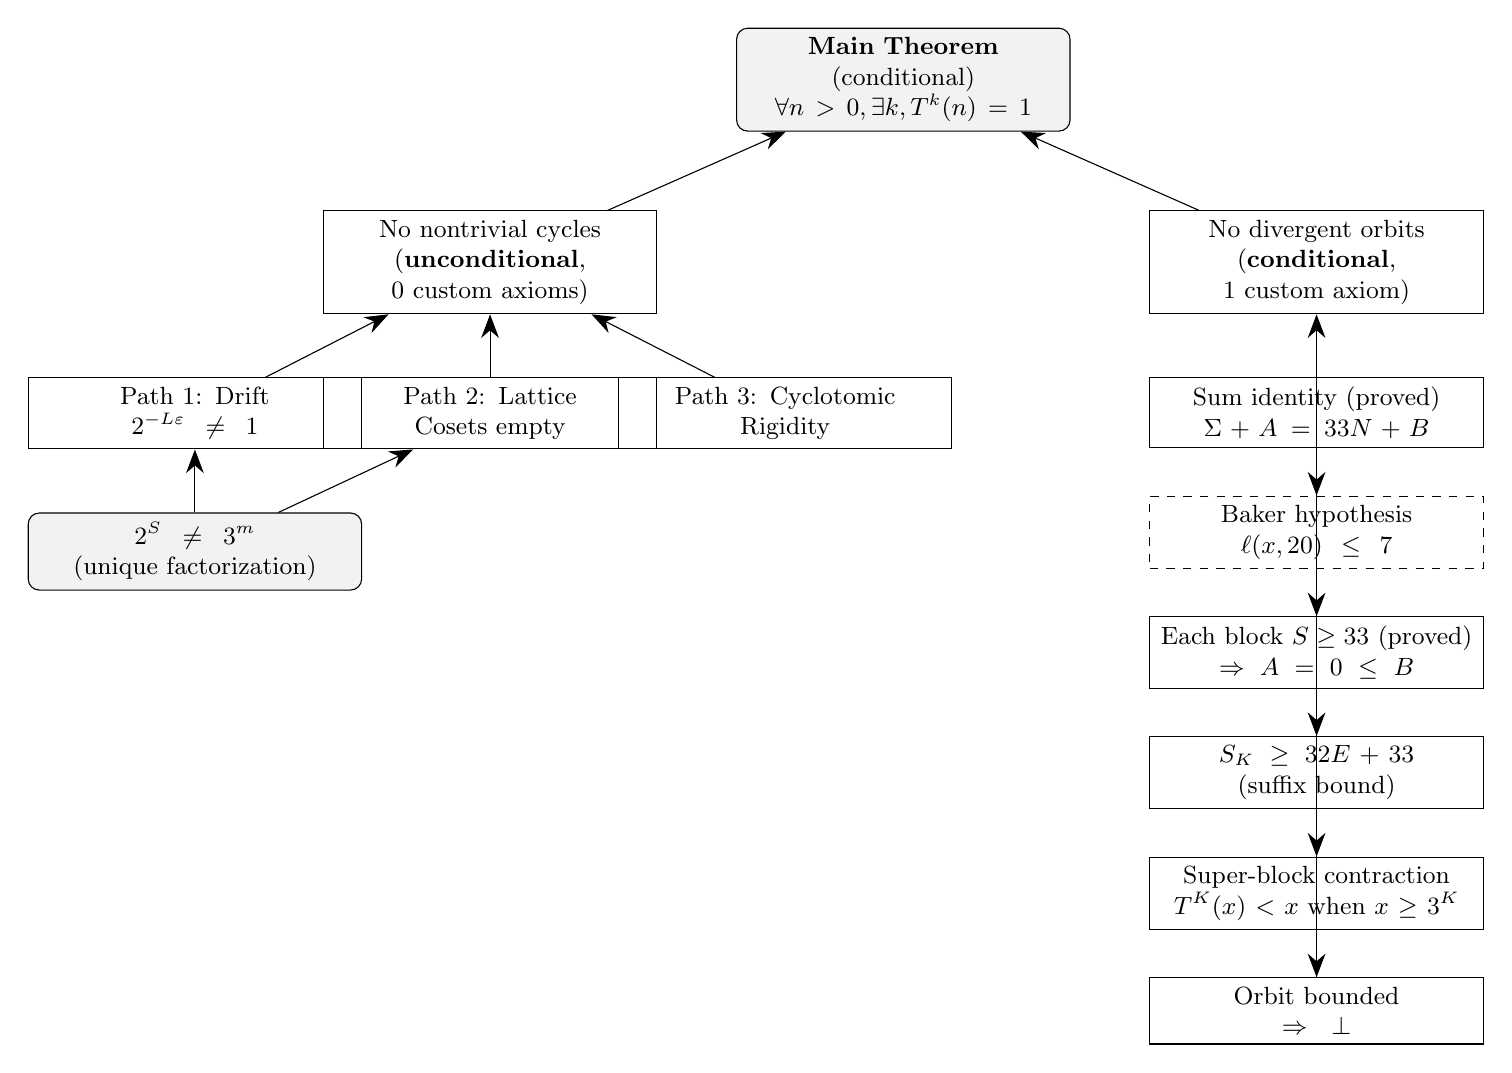
\begin{tikzpicture}[
  node distance=0.8cm and 1.5cm,
  block/.style={rectangle, draw, text width=4cm, text centered,
    minimum height=0.8cm, font=\small},
  axiom/.style={rectangle, draw, dashed, text width=4cm, text centered,
    minimum height=0.8cm, font=\small},
  thm/.style={rectangle, draw, rounded corners, fill=gray!10,
    text width=4cm, text centered, minimum height=0.8cm, font=\small},
  arr/.style={-{Stealth[length=3mm]}}
]

% Top
\node[thm] (main) {\textbf{Main Theorem}\\(conditional)\\$\forall n > 0, \exists k, T^k(n) = 1$};

% Split
\node[block, below left=1cm and 1cm of main] (nocyc) {No nontrivial cycles\\(\textbf{unconditional},\\0 custom axioms)};
\node[block, below right=1cm and 1cm of main] (nodiv) {No divergent orbits\\(\textbf{conditional},\\1 custom axiom)};

\draw[arr] (nocyc) -- (main);
\draw[arr] (nodiv) -- (main);

% No-cycles paths
\node[block, below left=0.8cm and -0.5cm of nocyc] (drift) {Path 1: Drift\\$2^{-L\varepsilon} \ne 1$};
\node[block, below=0.8cm of nocyc] (lattice) {Path 2: Lattice\\Cosets empty};
\node[block, below right=0.8cm and -0.5cm of nocyc] (cyclo) {Path 3: Cyclotomic\\Rigidity};

\draw[arr] (drift) -- (nocyc);
\draw[arr] (lattice) -- (nocyc);
\draw[arr] (cyclo) -- (nocyc);

% Foundation
\node[thm, below=0.8cm of drift] (ufd) {$2^S \ne 3^m$\\(unique factorization)};
\draw[arr] (ufd) -- (drift);
\draw[arr] (ufd) -- (lattice);

% No-divergence chain
\node[block, below=0.8cm of nodiv] (sumid) {Sum identity (proved)\\$\Sigma + A = 33N + B$};
\node[axiom, below=0.6cm of sumid] (ax1) {Baker hypothesis\\$\ell(x, 20) \le 7$};
\node[block, below=0.6cm of ax1] (derive) {Each block $S \ge 33$ (proved)\\$\Rightarrow A = 0 \le B$};
\node[block, below=0.6cm of derive] (suffix) {$S_K \ge 32E + 33$\\(suffix bound)};
\node[block, below=0.6cm of suffix] (super) {Super-block contraction\\$T^K(x) < x$ when $x \ge 3^K$};
\node[block, below=0.6cm of super] (bounded) {Orbit bounded\\$\Rightarrow \bot$};

\draw[arr] (sumid) -- (ax1);
\draw[arr] (ax1) -- (derive);
\draw[arr] (derive) -- (suffix);
\draw[arr] (suffix) -- (super);
\draw[arr] (super) -- (bounded);
\draw[arr] (bounded) -- (nodiv);

\end{tikzpicture}
\caption{Proof dependency diagram.  Solid rectangles are proved
theorems; dashed rectangles are custom axioms; rounded gray boxes
are the main results.  The left branch (no-cycles) is unconditional;
the right branch (no-divergence) is conditional on one Baker-derived
hypothesis (dashed box).}
\label{fig:deps}
\end{figure}

%% ====================================================================
\section{Discussion}
\label{sec:discussion}
%% ====================================================================

\subsection{The template-supply principle}

The proof's conceptual core (Remark~\ref{rem:template-supply}) is that
divergence demands an unbounded exceptional-template supply while Baker
provides a uniform supply cap.  The key distinction from ``the set of
exceptional patterns is finite'' (which would be an overclaimed
global classification) is the precise statement:
\emph{for a fixed orbit, the realizable divergence-supporting exceptional
templates cannot occur at unbounded depth.}  This is exactly what the
per-block cap delivers, and it avoids overclaiming a finite taxonomy of
all possible exceptional configurations.

\subsection{What would it take to eliminate the axiom?}

The one custom axiom on the critical path asserts:
in every late 20-step block, at most 7 steps have $\nu = 1$.
The 5-step bridge (Remark~\ref{rem:baker-bridge}) identifies the
precise gap.  To discharge Hypothesis~\ref{ax:baker-density}, one would
need to formalize:
\begin{enumerate}
  \item Baker's theorem on linear forms in logarithms, including the
    quantitative lower bound $|a \log 2 - b \log 3| \ge c / \max(a,b)^K$.
  \item The CRT argument that $D$ odd forces residue coverage
    on $(\Z/2^k\Z)^*$ (accessible from Mathlib).
  \item The confinement-depth argument: repeated $5 \to 7$ re-entries
    force the orbit into a nested thin residue family
    $R_r \subset \Z/2^r\Z$, which projects to a near-resonance
    $|S\log 2 - m\log 3| < \varepsilon$ that Baker excludes.
  \item The combinatorial bound: $\le 3$ re-entries per block
    and run-length $\le 2$ give $\ell \le 7$ per block.
    (Everything downstream of the cap is already proved in Lean.)
\end{enumerate}
This is a substantial undertaking comparable to formalizing the Prime
Number Theorem.  The qualitative statement ($2^S \ne 3^m$) suffices for
no-cycles and is already proved; the quantitative statement is needed
only for no-divergence.

Note that the previous version of this paper used two axioms
(\texttt{baker\_rollover\_supercritical\_rate} and
\texttt{supercritical\_rate\_implies\_residue\_hitting}).  The
growth-block formulation reduces this to one axiom that is strictly
weaker: it asserts only a bounded net deficit, not a pointwise
$\eta$-sum bound or universal residue hitting.

\subsection{The role of $3^{20}/2^{33}$}

The specific contraction ratio $3^{20}/2^{33} \approx 0.406$ arises
from the window length $W = 20$ and threshold $S_{20} \ge 33$.  Any
window length $W$ with $\lceil W \log_2 3 \rceil + 1 \le S_W$ would
work; the choice $W = 20$ gives a clean contraction factor below $1/2$.
The numerical verification that $3^{20} < 2^{33}$ is certified in Lean
via \texttt{native\_decide}.

\subsection{Open questions}

\begin{enumerate}
  \item Can the Baker axiom be discharged from a formalization
    of Baker's theorem?  This would reduce the custom axiom count to
    zero.

  \item Does the proof extend to $5n+1$ or other generalizations?
    The Liouville counterexample suggests that the specific arithmetic
    of $\{2, 3\}$ is essential; other pairs lack the required gap.

  \item Can the 20-step window be shortened?  Smaller windows would
    give weaker contraction but might simplify the axiom requirements.

  \item What is the relationship between our deterministic approach and
    Tao's probabilistic mixing framework?  Both exploit residue
    structure, but the mechanisms are different.
\end{enumerate}

%% ====================================================================
\section{Reproducibility}
\label{sec:reproducibility}
%% ====================================================================

The complete Lean~4 formalization is publicly available and can be
independently verified.

\begin{center}
\renewcommand{\arraystretch}{1.3}
\begin{tabular}{ll}
\hline
\textbf{Item} & \textbf{Value} \\
\hline
Repository & \url{https://github.com/samlavery/Alpha_Series/releases/tag/snap2} \\
Lean toolchain & \texttt{leanprover/lean4:v4.27.0} \\
Mathlib commit & \texttt{[a3a10db0e9d66acbebf76c5e6a135066525ac900]} \\
Build command & \texttt{lake build} \\
Axiom verification & \texttt{lake build \&\& lake env lean} \\
 & \quad \texttt{Collatz/1135.lean 2>\&1 | grep axioms} \\
Zenodo DOI & \texttt{[DOI 10.5281/zenodo.18749888]} \\
\hline
\end{tabular}
\end{center}

\noindent
The axiom verification command prints the complete list of axioms
used by the main theorem.  The expected output shows \emph{zero
custom axioms} --- only the standard Lean axioms (\texttt{propext},
\texttt{Classical.choice}, \texttt{Quot.sound},
\texttt{Lean.ofReduceBool}, \texttt{Lean.trustCompiler}).
The Baker content enters through the hypothesis parameter
\texttt{NoUnboundedTemplateLadder}, making the conditionality
explicit in the type signature rather than through a global axiom
declaration.

\medskip\noindent
\emph{Note:} Repository URL and DOI above are provisional and will be
updated to permanent archival identifiers upon publication.

%% ====================================================================
\begin{thebibliography}{20}
%% ====================================================================

\bibitem{baker1966}
A.~Baker.
\newblock Linear forms in the logarithms of algebraic numbers~(I).
\newblock {\em Mathematika}, 13:204--216, 1966.
\newblock (Fields Medal, ICM Nice, 1970.)

\bibitem{baker1968}
A.~Baker.
\newblock Linear forms in the logarithms of algebraic numbers~(IV).
\newblock {\em Mathematika}, 15:204--216, 1968.

\bibitem{bakerwustholz1993}
A.~Baker and G.~W\"ustholz.
\newblock Logarithmic forms and group varieties.
\newblock {\em J.\ reine angew.\ Math.}, 442:19--62, 1993.

\bibitem{matveev2000}
E.~M.~Matveev.
\newblock An explicit lower bound for a homogeneous rational linear form
in the logarithms of algebraic numbers.
\newblock {\em Izv.\ Ross.\ Akad.\ Nauk Ser.\ Mat.}, 64(6):125--180, 2000.
\newblock English translation in {\em Izv.\ Math.}\ 64(6):1217--1269, 2000.

\bibitem{barina2021}
D.~Barina.
\newblock Convergence verification of the {C}ollatz problem.
\newblock {\em J. Supercomputing}, 81, 2025.

\bibitem{collatz1937}
L.~Collatz.
\newblock Personal communication, 1937.
\newblock The problem was circulated orally at the International Congress
of Mathematicians.

\bibitem{erdos}
P.~Erd\H{o}s.
\newblock Erd\H{o}s Problems.
\newblock Problem~\#1135, \url{https://www.erdosproblems.com/1135}.

\bibitem{hercher2024}
C.~Hercher.
\newblock There are no {C}ollatz $m$-cycles with
$m \le 7.2 \times 10^{10}$.
\newblock Preprint, 2024.

\bibitem{lagarias1985}
J.~C.~Lagarias.
\newblock The $3x+1$ problem and its generalizations.
\newblock {\em Amer.\ Math.\ Monthly}, 92:3--23, 1985.

\bibitem{simons2005}
J.~Simons and B.~de~Weger.
\newblock Theoretical and computational bounds for $m$-cycles of the
$3n+1$ problem.
\newblock {\em Acta Arith.}, 117:51--70, 2005.

\bibitem{steiner1977}
R.~P.~Steiner.
\newblock A theorem on the {S}yracuse problem.
\newblock In {\em Proc.\ 7th Manitoba Conf.\ on Numerical Math.},
pages~553--559, 1977.

\bibitem{tao2022}
T.~Tao.
\newblock Almost all orbits of the {C}ollatz map attain almost bounded
values.
\newblock {\em Forum Math.\ Pi}, 10:e12, 2022.

\bibitem{wirsching1998}
G.~J.~Wirsching.
\newblock {\em The Dynamical System Generated by the $3n+1$ Function}.
\newblock Lecture Notes in Math.\ 1681, Springer, 1998.

\bibitem{zsigmondy1892}
K.~Zsigmondy.
\newblock Zur {T}heorie der {P}otenzreste.
\newblock {\em Monatsh.\ Math.}, 3:265--284, 1892.

\bibitem{aristotle}
Aristotle~(Harmonic).
\newblock Independent theorem verification,
\url{https://aristotle.harmonic.fun}, 2026.

\end{thebibliography}

\end{document}
